\documentclass[conference]{IEEEtran}
% IEEEtran.cls: the copy supplied with the IEEE conference template (6/27/2024).

\usepackage{cite}
\usepackage{amsmath,amssymb,amsfonts}
\usepackage{graphicx}
\usepackage{textcomp}
\usepackage{xcolor}
\usepackage{booktabs}
\usepackage{array}

\graphicspath{{../figures/glover37/}}

% Every run-of-record number in the text is a macro generated from
% results/glover37/analysis/summary.csv (written by the report stage).
% Generated by experiments/glover37/report.py from analysis/summary.csv and
% validation/summary.csv. Do not edit; rerun the report stage.
\newcommand{\NumWeekStart}{12 November 2025, 17:00}
\newcommand{\NumLoadScaleMin}{0.70}
\newcommand{\NumLoadScalePeak}{1.24}
\newcommand{\NumUnitsFewestNoIBR}{4}
\newcommand{\NumUnitsMostNoIBR}{7}
\newcommand{\NumUnitsFewestIBR}{3}
\newcommand{\NumUnitsMostIBR}{7}
\newcommand{\NumLinesOut}{42}
\newcommand{\NumLinesAll}{42}
\newcommand{\NumTransformersOut}{14}
\newcommand{\NumTransformersAll}{14}
\newcommand{\NumCorridors}{48}
\newcommand{\NumStates}{9,744}
\newcommand{\NumConeIntact}{10 of 10}
\newcommand{\NumConeAll}{472 of 490}
\newcommand{\NumConeZonly}{490 of 490}
\newcommand{\NumConeExceptions}{18}
\newcommand{\NumConeExceptionHourFirst}{5}
\newcommand{\NumConeExceptionHourLast}{6}
\newcommand{\NumConeExceptionUnits}{5}
\newcommand{\NumConeExceptionGap}{0.29\,\%}
\newcommand{\NumConeRangeLow}{14.3\,\%}
\newcommand{\NumConeRangeHigh}{47.2\,\%}
\newcommand{\NumCtwoLoadLow}{0.97}
\newcommand{\NumCtwoLoadHigh}{1.24}
\newcommand{\NumCtwoZonlyHour}{9}
\newcommand{\NumCtwoDeltaVLow}{$-$0.099}
\newcommand{\NumCtwoDeltaVHigh}{$-$0.025}
\newcommand{\NumCtwoDeltaZLow}{0.004}
\newcommand{\NumCtwoDeltaZHigh}{0.015}
\newcommand{\NumCtwoRangeLow}{1.2\,\%}
\newcommand{\NumCtwoRangeHigh}{8.8\,\%}
\newcommand{\NumCthreeGapEone}{0.78\,\%}
\newcommand{\NumCthreeGapEfiveMin}{8.75\,\%}
\newcommand{\NumCthreeGapEfiveWorse}{0.67\,\%}
\newcommand{\NumCfourHoursEone}{7, 8}
\newcommand{\NumCfourSpanEfive}{67 h}
\newcommand{\NumCfiveNetMax}{0.30\,\%}
\newcommand{\NumCfiveNetMin}{$-$63\,\%}
\newcommand{\NumCsixCorrSCR}{0.995}
\newcommand{\NumCsixCorrWSCR}{0.990}
\newcommand{\NumCsevenCorrESCR}{0.790}
\newcommand{\NumCsevenCorrSDSCR}{0.709}
\newcommand{\NumCsevenOppESCR}{499}
\newcommand{\NumCsevenOppSDSCR}{494}
\newcommand{\NumCsevenShareESCR}{2.1\,\%}
\newcommand{\NumCsevenShareSDSCR}{2.0\,\%}
\newcommand{\NumCsevenMaxESCR}{6.52\,\%}
\newcommand{\NumCsevenMaxSDSCR}{4.40\,\%}
\newcommand{\NumCsevenVoneESCR}{504}
\newcommand{\NumCsevenVoneSDSCR}{504}
\newcommand{\NumCsevenNoIntESCR}{0}
\newcommand{\NumCsevenNoIntSDSCR}{0}
\newcommand{\NumCeightImpShare}{2.1\,\%}
\newcommand{\NumCeightImpMax}{6.5\,\%}
\newcommand{\NumCeightProbeHalfShare}{16.9\,\%}
\newcommand{\NumCeightProbeOneShare}{20.0\,\%}
\newcommand{\NumCeightProbeTwoShare}{22.0\,\%}
\newcommand{\NumCeightProbeOneMax}{67.1\,\%}
\newcommand{\NumCeightProbeOneSameHour}{80 of 147}
\newcommand{\NumCnineParallel}{80 of 80}
\newcommand{\NumCnineParallelDln}{0.0029}
\newcommand{\NumFthreeBeyondSCR}{1046}
\newcommand{\NumFthreeBeyondWSCR}{182}
\newcommand{\NumFthreeBeyondESCR}{328}
\newcommand{\NumFthreeBeyondSDSCR}{320}
\newcommand{\NumFthreeLowestSCR}{$-$63\,\%}
\newcommand{\NumPowerWorldMaxErrorPct}{0.0074}
\newcommand{\NumOutages}{56}
\newcommand{\NumCases}{49}


\begin{document}

\title{Evaluating Fault-Current System Strength Metrics under Time-Varying Operation and N-1 Contingencies}


\author{\IEEEauthorblockN{1\textsuperscript{st} Leandro Morita}
\IEEEauthorblockA{\textit{Department of Electrical Engineering, Division of Electricity} \\
\textit{Uppsala University}\\
Uppsala, Sweden \\
leandro.morita@angstrom.uu.se}
\and
\IEEEauthorblockN{2\textsuperscript{nd} Robert Eriksson}
\IEEEauthorblockA{\textit{Department of Electrical Engineering, Division of Electricity} \\
\textit{Uppsala University}\\
Uppsala, Sweden \\
robert.eriksson@angstrom.uu.se}
}

\maketitle

\begin{abstract}
System-strength screening metrics help decide which inverter-based resource (IBR) connections and operating conditions require detailed electromagnetic-transient (EMT) studies. Each metric is specified with its own network model, evaluation point and interaction factor, and the metrics have been compared only on discrete cases.
This paper shows that SCR, WSCR, ESCR and SDSCR are built from the same quantities: the pre-fault voltage, the driving-point impedance and an interaction term.
Unlike earlier comparisons, the metrics are followed through a time-ordered sequence of operating states, and each change is split exactly into these parts, so any difference can be traced to the metrics themselves or to their conventions.
Three IBR plants on a 37-bus benchmark are studied over a week, with load following a public demand profile, intact and under every single line and transformer outage.
Wherever synchronous-generator commitment varies, it sets the weakest hour for all four metrics. Under outages, the metrics follow the change in network impedance; ESCR and SDSCR oppose it only rarely, while ESCR does so far more often when its interaction factor includes generator voltage control.
Screening over time therefore needs a model of commitment, and ESCR values should state how the interaction factor is obtained.
\end{abstract}

\begin{IEEEkeywords}
grid strength, system strength, inverter-based resources, short-circuit ratio, screening, unit commitment, contingency analysis
\end{IEEEkeywords}

\section{Introduction}
\label{sec:introduction}

As inverter-based resources (IBRs) displace synchronous generation, the strength of the grid at
their connection points becomes a planning concern \cite{SvK2025, fingrid2023, Denholm2022, NERC2018}. Fault-current-based metrics are the
usual first screen: they are quick to compute from a network model, and their values decide
which connections and operating conditions receive detailed electromagnetic-transient study
\cite{ieee2800,nerc2017,cigre671}. IEEE Std 2800-2022 adds that a value used across a system
should cover a variety of operating conditions and topologies \cite{ieee2800}. Screening is
therefore only as reliable as the metric's ability to identify when, and under which outages, a
site is weakest.

Several such metrics are in use, and each comes with its own conventions. The short-circuit ratio
(SCR) and the weighted SCR (WSCR) are evaluated at the point of interconnection on the network
without the IBR plants \cite{ieee2800,zhang2014}. The equivalent SCR (ESCR), titled SCRIF in IEEE
Std 2800-2022 \cite{ieee2800,cigre671}, adds the plants' interaction through multi-infeed interaction
factors \cite{cigre364}, and is applied on the medium-voltage side \cite{fingrid2023}. The
site-dependent SCR (SDSCR) weights the other plants through the impedance matrix at the converter
terminals \cite{wu2018}. Names and the construction of the interaction factor differ between
sources \cite{joswigjones2026,goonasekara2023,darii2026}. Comparisons of the metrics so far rest
on discrete cases: Wu et al. \cite{wu2018} compare them over twelve operating and
contingency conditions, others use a handful of loading cases or single snapshots
\cite{sanni2022,dhungana2026,khamees2026,rosengren2025}, and commitment has been shown to drive
WSCR within a single period \cite{kim2025}. WSCR, however, is a group metric and does not give the strength of individual sites.
To the authors' knowledge, no study has followed the
metrics through a time-ordered sequence of operating states, in which commitment changes with
load, together with a full set of line and transformer outages.

This paper asks whether SCR, WSCR, ESCR and SDSCR, each applied as specified, lead to consistent
screening conclusions along such a sequence, and what explains any difference. Over time, it asks
whether the metrics agree on when each site is weakest, whether any metric tells more than the
committed set of synchronous generators, and whether the usual planning snapshots find the weekly
minimum. Under outages, it asks what a single branch outage does to each site. Finally, it asks whether
differences come from the metrics themselves or from their conventions (network model, evaluation
point and interaction-factor construction).

The study adds three IBR plants to the 37-bus network of \cite{gloverPSAD} and evaluates the four metrics over
a 168-hour week, with load scaled by a public demand profile, under a largest-first commitment rule,
intact and for each single line and transformer outage, and with every unit online on the intact
network. The contributions are:
\begin{itemize}
  \item a time-ordered, per-site comparison of the four metrics over a week and the full N-1 branch
        set, each under its practitioner-specified network, evaluation point and denominator;
  \item an attribution of every agreement and disagreement to a term of the metric, confirmed by
        removing that term or holding it constant;
  \item a reconciliation of the metrics' conventions, including how the choice of interaction
        factor changes ESCR's response to outages;
  \item a reproducible implementation on public data and open code.
\end{itemize}

Section~\ref{sec:metrics} defines the metrics and their conventions, and Section~\ref{sec:study}
the benchmark, operating states and experiments. Section~\ref{sec:results} presents the results,
Section~\ref{sec:discussion} discusses their implications and limitations, and
Section~\ref{sec:conclusion} concludes.

\section{Metrics and Conventions}
\label{sec:metrics}

\subsection{Fault quantities}

All four metrics are built from the short-circuit power and the impedance matrix at the evaluation
bus. For bus $i$ in a given network and operating state, the short-circuit power $\mathrm{SCMVA}_i$ (MVA) is
obtained from a bolted three-phase fault solved from the actual pre-fault power flow, with
$\mathrm{SCMVA}_i = S_\mathrm{b}|I_{\mathrm{f},i}|$ at $V_\mathrm{n} = 1$~pu and $S_\mathrm{b} = 100$~MVA. The
impedance matrix $\mathbf{Z} = \mathbf{Y}^{-1}$ comes from the same fault model: the passive
network, the source admittances of the committed synchronous generators, and constant-impedance
equivalents of the loads at their pre-fault voltages. Assuming constant-impedance loads and constant-current
converters during the fault, the fault network is linear, and
$\mathrm{SCMVA}_i \approx S_\mathrm{b}|V_i|/|Z_{ii}|$: the short-circuit power carries both the driving-point
impedance $Z_{ii}$ and the pre-fault voltage magnitude $|V_i|$. Every denominator uses the IBR plants' rated active
power $P_i$.

\subsection{Metrics}

Table~\ref{tab:conventions} lists the four metrics, each with the network, evaluation point and
interaction term its source specifies; Section~\ref{sec:study} gives the plant model and where each
point lies in it. SCR and WSCR are evaluated at the point of interconnection (POI), on the
transmission network without the IBR plants \cite{ieee2800}; WSCR combines the three sites into one
group value \cite{ieee2800,zhang2014}. ESCR is evaluated at each plant's medium-voltage (MV) bus,
the high-voltage side of its padmount transformer, on the network with the IBR plants
\cite{fingrid2023}. It is the multi-infeed ESCR of
\cite{cigre364} with no reactive compensation, the quantity titled SCRIF in \cite{ieee2800} and
equivalent SCR in \cite{cigre671,fingrid2023}; it is not the effective SCR of line-commutated HVDC,
which subtracts filter reactive power. SDSCR is evaluated at the converter terminal, on the low-voltage
side of the padmount transformer, as in \cite{wu2018}. Its weights $w_{ij}$ are complex, with the conjugated
voltage ratio as in \cite{wu2018,maharjan2023}, and
the magnitude is taken of the whole weighted sum.

\begin{table}[!t]
\caption{Metric definitions and conventions}
\label{tab:conventions}
\centering
\footnotesize
\setlength{\tabcolsep}{3pt}
\begin{tabular}{@{}llllc@{}}
\toprule
Metric & Definition & IBR & Point & Ref. \\
\midrule
SCR & $S_i / P_i$ & no & POI & \cite{ieee2800} \\
WSCR & $\sum_i S_i P_i \,/\, (\sum_i P_i)^2$ & no & POI & \cite{ieee2800} \\
ESCR & $S_i \,/\, (P_i + \sum_{j \ne i} \mathrm{MIIF}_{ji} P_j)$ & yes & MV bus & \cite{cigre364} \\
SDSCR & $|V_i|^2 \,/\, (|Z_{ii}|\,|P_i + \sum_{j \ne i} w_{ij} P_j|)$ & yes & converter terminal & \cite{wu2018} \\
\midrule
\multicolumn{5}{@{}p{\linewidth}@{}}{\scriptsize $\mathrm{MIIF}_{ji} = |Z_{ji}/Z_{ii}|$; $w_{ij} = (Z_{ij}/Z_{ii})\,(V_i/V_j)^*$; $Q_f = 0$ in ESCR; $P$: rated active power.} \\
\bottomrule
\end{tabular}

\end{table}

\subsection{Interaction factor}

ESCR and SDSCR add an interaction term to the plant's own power: $\sum_{j\ne i}
\mathrm{MIIF}_{ji}P_j$ and $\sum_{j\ne i} w_{ij}P_j$, respectively. SCR and WSCR have none. The
multi-infeed interaction factor $\mathrm{MIIF}_{ji}$ is the ratio of the voltage changes
$\Delta V_j/\Delta V_i$ for a small voltage step at bus $i$ \cite{cigre364}. The step is about
1\,\%, small enough that no voltage-controlling device acts, and the ratio then equals the
impedance-matrix form $|Z_{ji}/Z_{ii}|$ \cite{cigre364}. This impedance form is the reference used
here. Other sources obtain the factor differently: IEEE Std 2800-2022 \cite{ieee2800} allows impedance-matrix
manipulation or reactive-power injection, and Fingrid \cite{fingrid2023} applies a voltage step in a power
flow, in which voltage-regulating generators respond. Section~\ref{sec:study} describes the
voltage-step variant used to test this choice.

\subsection{Attribution of changes}

All four metrics share one structure. With the approximation of Section~\ref{sec:metrics}-A,
SCR, ESCR and SDSCR can be written as
\begin{equation}
m \approx \frac{S_\mathrm{b}\,|V_i|^{a}}{|Z_{ii}|\,D_i} ,
\label{eq:shape}
\end{equation}
exactly for SDSCR, with the exponent $a$ and the denominator $D_i$ in Table~\ref{tab:shape}.
\begin{table}[!t]
\caption{Exponent and denominator of each metric in \eqref{eq:shape}}
\label{tab:shape}
\centering
\footnotesize
\renewcommand{\arraystretch}{1.3}
\begin{tabular}{@{}lcl@{}}
\toprule
Metric & $a$ & $D_i$ \\
\midrule
SCR & 1 & $P_i$ \\
ESCR & 1 & $P_i + \sum_{j\ne i}\mathrm{MIIF}_{ji}P_j$ \\
SDSCR & 2 & $|P_i + \sum_{j\ne i} w_{ij}P_j|$ \\
\bottomrule
\end{tabular}
\end{table}
WSCR is a weighted sum of the three sites' SCRs, with fixed weights $(P_i/\sum_k P_k)^2$. With $P_i$ the rated power in every state, the
change of a metric between two states (two hours, or an outage and the intact case) splits into
three parts:
\begin{equation}
\Delta\ln m = \underbrace{a\,\Delta\ln|V_i|}_{\delta_V}
\;\underbrace{-\,\Delta\ln D_i}_{\delta_I}
\;\underbrace{-\,\Delta\ln|Z_{ii}|}_{\delta_Z} ,
\label{eq:split}
\end{equation}
the pre-fault-voltage, interaction and driving-point-impedance parts,
$\delta_V = a\,\Delta\ln|V_i|$, $\delta_I = -\Delta\ln D_i$ and $\delta_Z = -\Delta\ln|Z_{ii}|$,
each positive when it raises the metric. The interaction part is zero
for SCR and WSCR. Since~\eqref{eq:shape} is approximate, the parts are computed exactly by recomputing the metric
with unit pre-fault voltage and without the interaction factor. A site is called weaker when its
metric falls, and the network weaker when $|Z_{ii}|$ rises ($\delta_Z < 0$).

\section{Study Design}
\label{sec:study}

\subsection{Network and IBR plants}

The study uses the 37-bus network of \cite{gloverPSAD}: 37 buses, 42 lines, 14 transformers, 26
loads totalling 806~MW and 281~Mvar, seven synchronous generators plus a slack at bus 31, and a 100-MVA base. Three IBR
plants of 60, 45 and 45~MW are connected at their POIs, the 69-kV buses 21, 48 and 16
(Fig.~\ref{fig:network}). Each plant is modelled as in Fig.~\ref{fig:plant}: a 69/34.5-kV main
transformer, a collector feeder to the MV bus, a 34.5/0.69-kV padmount transformer and one
aggregate converter. Following \cite{dhungana2026}, the converter is rated at 1.1 times the
plant's active power and each transformer at 1.2 times the converter rating, with
$0.005 + j0.06$~pu on its own base. The converters inject their rated active power at unity
power factor in every state, the case in which they displace the most synchronous generation.
Adding the plants gives the 46-bus network on which ESCR and SDSCR
are evaluated; SCR and WSCR use the 37-bus network without them (Table~\ref{tab:conventions}).

\begin{figure}[!t]
\centering
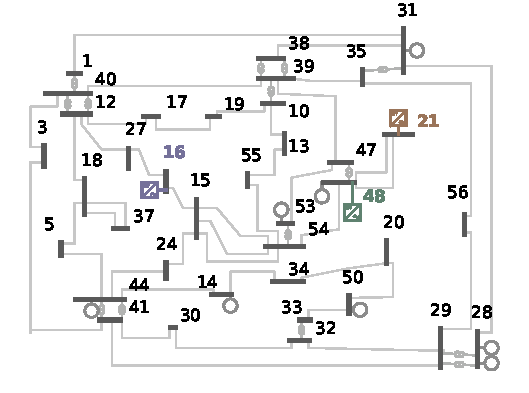
\includegraphics[width=\linewidth]{f1a_network}
\caption{The 37-bus network with the three IBR plants at buses 21, 48 and 16.}
\label{fig:network}
\end{figure}

\begin{figure}[!t]
\centering
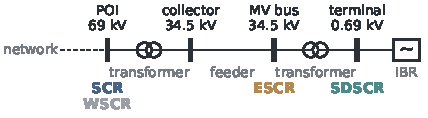
\includegraphics[width=0.85\linewidth]{f1b_plant}
\caption{Model of one IBR plant and the evaluation point of each metric: POI, MV bus and
converter terminal.}
\label{fig:plant}
\end{figure}

\subsection{Operating states}

Public hourly demand for the Swedish bidding zone SE3 in 2025 serves only as a scaling signal.
The 168-hour window with the largest load range, starting \NumWeekStart~UTC, scales
every load's active and reactive power by the hourly demand divided by the window mean. The load
scale ranges from \NumLoadScaleMin{} to \NumLoadScalePeak.

Generation is committed by one of two rules. Under the largest-first rule, the non-slack units
are committed in descending order of maximum output, each within its limits, until the remaining
demand is below the next unit's minimum output; the slack takes the rest. With every unit online,
all non-slack units run at a common fraction of their maximum output, not below their minimum,
and the slack takes the rest. The 37-bus network dispatches the full demand and the 46-bus
network the demand less the IBR plants' 150~MW, each with its own schedule. Under the largest-first
rule, between \NumUnitsFewestNoIBR{} and \NumUnitsMostNoIBR{} units are committed on the 37-bus
network and between \NumUnitsFewestIBR{} and \NumUnitsMostIBR{} on the 46-bus network. Each
state is a Newton--Raphson power flow with generator reactive limits and the case's automatic tap
controllers; the IBR transformers keep nominal taps.

\subsection{Branch outages}

Every line and transformer of the 37-bus network whose outage islands no bus and leaves both
networks solvable in all 168 hours is outaged in turn: \NumLinesOut{} of the \NumLinesAll{} lines
and \NumTransformersOut{} of the \NumTransformersAll{} transformers. The IBR plants' own transformers are not outaged,
since that would disconnect the plant. Commitment and dispatch are held at the intact schedule, so an outage changes only the topology. The pre-fault voltages then follow from the power flow. 
The \NumOutages{} outages fall into \NumCorridors{} corridors, since parallel branches count once
(lines 18--37, 21--48 and 15--54; transformers 12--40, 28--29, 38--39 and 41--44).

\subsection{Experiments and validation}

The metrics are evaluated on three sets of states, \NumStates{} in all: the intact week under the
largest-first rule, the same week under each branch outage, and the intact week with every unit
online.

To test the interaction-factor convention, ESCR is also computed on the first two sets with a
voltage-step factor in place of the impedance-based reference. An ideal voltage source with zero
active power at bus $i$ raises $|V_i|$ by a step of 0.5, 1 or 2\,\% in a power flow started
from the solved state, with taps frozen and the generators regulating their voltages. The factor
$\mathrm{MIIF}_{ji} = \Delta V_j/\Delta V_i$ then includes their response.

The fault calculation was checked against PowerWorld on the base case
and six other network configurations with generator, line or transformer changes, with fault currents agreeing within \NumPowerWorldMaxErrorPct\,\%.

\section{Results}
\label{sec:results}

\begin{figure}[!t]
\centering
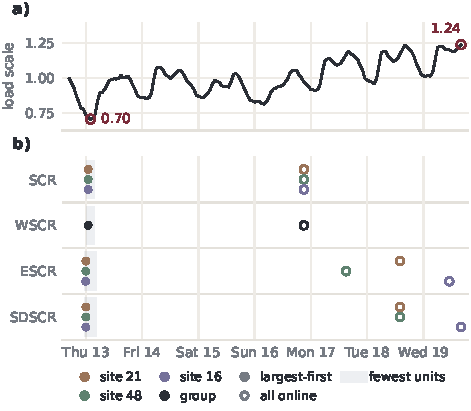
\includegraphics[width=\linewidth]{f2_week}
\caption{Intact week. (a) Load scale, with the minimum- and peak-load hours. (b) Hour at which
each metric is lowest at each site, under the largest-first rule (filled) and with every unit
online (open); minimum-commitment hours shaded.}
\label{fig:week}
\end{figure}

\subsection{When each site is weakest}

Under the largest-first rule, commitment follows load (Fig.~\ref{fig:week}): the fewest units
are online around the minimum-load hour, and commitment never falls as load rises. The results
are counted over ten metric--site pairs, three sites each for SCR, ESCR and SDSCR and one group
value for WSCR, and over \NumCases{} cases, the intact network and the \NumCorridors{} corridors. The
weekly minimum falls in these minimum-commitment hours in \NumConeAll{} pair--case
combinations (Fig.~\ref{fig:week}b). The cause is the driving-point impedance: with fewer
generators committed, fewer source admittances lie in parallel and $|Z_{ii}|$ rises. With $\delta_Z$ isolated
in~\eqref{eq:split} ($\delta_V$ and $\delta_I$ set to zero), every combination has its weakest
hour in these hours. The
\NumConeExceptions{} exceptions, all SCR or WSCR under outages, are combinations in which the change in the pre-fault voltage $\delta_V$
slightly outweighs the change in the driving-point impedance $\delta_Z$ in~\eqref{eq:split}.

With every unit online throughout the intact week, commitment no longer changes and the weakest hour moves to high load, at
load scales of \NumCtwoLoadLow{} to \NumCtwoLoadHigh. The pre-fault voltage falls as load rises,
and in every pair $\delta_V$ outweighs $\delta_Z$ in~\eqref{eq:split}. The driving-point
impedance changes only through the loads, which the fault model represents as constant
impedances (Section~\ref{sec:metrics}-A), so with $\delta_Z$ isolated the weakest hour would be at
minimum load (hour \NumCtwoZonlyHour). From that hour to the actual weakest hour, however, the
voltage part reduces the metric ($\delta_V$ from \NumCtwoDeltaVLow{} to \NumCtwoDeltaVHigh) more than the impedance part
raises it ($\delta_Z$ from \NumCtwoDeltaZLow{} to \NumCtwoDeltaZHigh). The metrics then vary much less: each pair's weekly maximum exceeds its
minimum by \NumCtwoRangeLow{} to \NumCtwoRangeHigh, against \NumConeRangeLow{} to
\NumConeRangeHigh{} under the largest-first rule. Their weakest hours, however, spread over
\NumCfourSpanEfive, within which each metric rises by a median of \NumCfourWindowMedian{} above
its weekly minimum (at most \NumCfourWindowMax, \NumCfourWindowMaxMetric). With commitment
fixed, the metrics thus disagree on the weakest hour.

Commitment thus sets the weakest hour wherever it varies, and otherwise the pre-fault voltage does, though the metrics then vary far less over the week.
This also explains the planning snapshots. Under the largest-first rule the
minimum-load hour is a minimum-commitment hour, and its snapshot lies within
\NumCthreeGapEone{} of the true minimum. With every unit online, the minimum-load snapshot
misses the true minimum by up to \NumCthreeGapEfiveMin.

\begin{figure*}[!t]
\centering
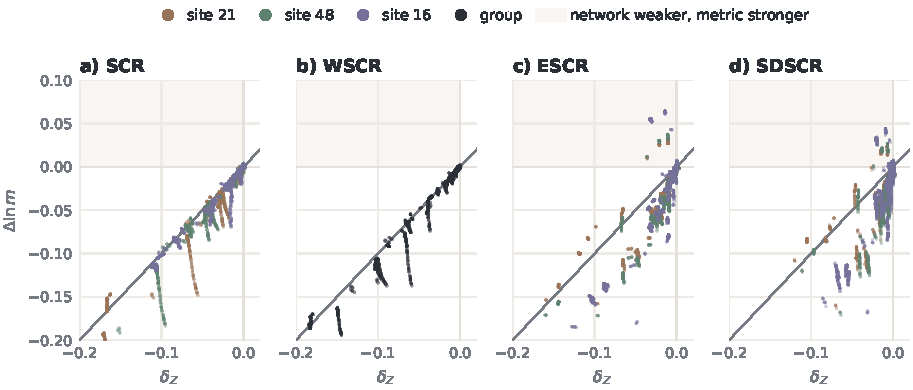
\includegraphics[width=\textwidth]{f3_outage}
\caption{Change $\Delta\ln m$ of each metric under a branch outage against its
driving-point-impedance part $\delta_Z$ in~\eqref{eq:split}, per point: (a) SCR, (b) WSCR,
(c) ESCR, (d) SDSCR. Shaded: network weaker, metric stronger. Points below $-0.2$ are not drawn (\NumFthreeBeyondSCR,
\NumFthreeBeyondWSCR, \NumFthreeBeyondESCR{} and \NumFthreeBeyondSDSCR{} points; lowest
\NumFthreeLowestSCR, SCR).}
\label{fig:outage}
\end{figure*}

\subsection{What a branch outage does}

Results under outages are counted per point, one corridor, hour and site: \NumPoints{} points per
metric, and \NumPointsGroup{} for the WSCR group value. An outage weakens the network or leaves it practically unchanged: $\delta_Z$ never exceeds
\NumCfiveDeltaMax{} (\NumCfiveNetMax), while it reaches \NumCfiveDeltaMin{} (\NumCfiveNetMin) at
worst. Fig.~\ref{fig:outage} plots each metric's change against this network change.
SCR and WSCR follow it, with no point more
than 1\,\% stronger; their points below the diagonal are those in which the pre-fault voltage
falls as well. ESCR and SDSCR follow it less closely and occasionally oppose it:
\NumCsevenOppESCR{} and \NumCsevenOppSDSCR{} points (\NumCsevenShareESCR{} and
\NumCsevenShareSDSCR) are more than 1\,\% stronger while
the network weakens, by at most \NumCsevenMaxESCR{} and \NumCsevenMaxSDSCR. 
All such points come from outages of a line at another plant's POI. The outage moves that plant
electrically away from the site, so its interaction factor falls and $\delta_I$ outweighs
$\delta_Z$ in~\eqref{eq:split}.
With $\delta_I$ set to zero, no point remains more than 1\,\% stronger, while with $\delta_V$ set to zero they remain. The
opposition thus comes from the interaction term in the metrics' definitions, not from a
convention.

\begin{figure}[!t]
\centering
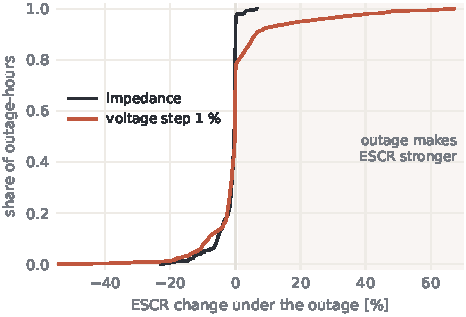
\includegraphics[width=\linewidth]{f4_interaction_factor}
\caption{Cumulative share of points by ESCR's change under an outage, with the
impedance-based interaction factor and the 1\,\% voltage step with generators regulating.
Shaded: more than 1\,\% stronger.}
\label{fig:miif}
\end{figure}

\subsection{How the interaction factor changes ESCR}

Fig.~\ref{fig:miif} compares ESCR's outage change under the impedance-based interaction factor
and under the 1\,\% voltage step. With the impedance form, ESCR is more than 1\,\%
stronger in \NumCsevenShareESCR{} of the points, as found in Section~\ref{sec:results}-B. With the
1\,\% voltage step, the share rises to \NumCeightProbeOneShare, and ESCR is up to \NumCeightProbeOneMax{}
stronger.
Using steps of 0.5 and 2\,\%, the share is \NumCeightProbeHalfShare{} and \NumCeightProbeTwoShare. A likely cause is the generators' voltage control. In
the voltage step, generators that regulate their terminal voltages hold the voltage near the
other plants, so $\Delta V_j$, and with it $\mathrm{MIIF}_{ji} = \Delta V_j/\Delta V_i$, is smaller
than in the impedance form, which contains no such response. $D_i$ then falls and ESCR rises. ESCR's response to
outages thus depends on how its interaction factor is obtained.

\section{Discussion and Limitations}
\label{sec:discussion}

Under the largest-first rule the four metrics agree on when each site is weakest: all reach
their minimum in the minimum-commitment hours, and no metric tells more than the committed set
of synchronous generators. With every unit online they disagree, although each then varies by
only a few percent over the week. The two rules, however,
place the weakest hour at opposite ends of the load range. The critical hour is thus a property
of the commitment, not of the metric, and a screen over time needs a model of commitment or
measured operating states. A minimum-load snapshot finds the weekly minimum where, as under
the largest-first rule here, the fewest units are online at minimum load.

Under outages, commitment still sets the weakest hour in nearly every case, and the outage
changes how weak the site is rather than when. The metrics differ in how they report that
change. SCR and WSCR follow the change in the network.
ESCR and SDSCR add the other plants' contribution, weighted by their electrical proximity to the site,
and an outage that moves another plant away lowers that weight. All the points in which they
oppose the network come from two outages, each of a line at another plant's POI, and the
interaction term alone explains them. A screen based on ESCR or SDSCR would therefore not flag
these outages, while one based on SCR would. Whether the site is in fact weaker or stronger 
cannot be decided from fault quantities, since both readings follow from the same impedances. 
It depends on whether the site's stability is limited more by the network's fault current or 
by the interaction between nearby plants, which only an EMT study can show.

The opposition found above does not come from a convention but from the interaction term in the
metrics' definitions. How the interaction factor is obtained, however, changes how often ESCR
opposes the network and by how much. Since the literature obtains it in different ways \cite{cigre364,ieee2800,fingrid2023}, an ESCR value should state how its
interaction factor is obtained.

The findings rest on the following modelling choices. The fault model assumes constant-impedance loads and
constant-current converters, which makes the fault network linear and \eqref{eq:shape} close to
exact. Converters that inject reactive current during the fault would make it nonlinear and add
their own contribution to the short-circuit power. The constant-impedance loads are also the only
path by which $|Z_{ii}|$ changes with load when every unit is online, so that result depends on
the load model. The voltage-step factor uses ideal voltage-controlled generators, so it remains
untested whether its smaller interaction comes from the network or from the ideal control, and
its dependence on the step size is not explained. The study covers one network and one week,
with the IBR plants at rated output and unity power factor, switched shunts fixed, commitment
held during outages and single branch outages only. Pre-fault voltages were not corrected to an
operating band. Since every plant runs at rated output, denominators based on rated, actual or
apparent power differ only by one constant factor per site and change no conclusion. The 1\,\%
threshold for a material change is a choice. The metric equations follow their sources, but the
computed values could not be checked against a published case.

\section{Conclusion}
\label{sec:conclusion}

SCR, WSCR, ESCR and SDSCR were followed through a week of operating states on a 37-bus benchmark
with three IBR plants, intact and under every single line and transformer outage, and each
change was split into its voltage, interaction and driving-point-impedance parts. Wherever
commitment varies, the four metrics agree on when each site is weakest, and commitment sets that
hour. With commitment fixed they disagree on the hour, although each varies little over the
week. No metric tells more than the committed set of generators, and the
minimum-load snapshot finds the weekly minimum when the fewest units run at minimum load, as under the
largest-first rule.
Under outages, SCR and WSCR follow the change in the network, while ESCR and SDSCR occasionally
report a site stronger while the network weakens. This follows from their interaction term, not
from a convention, although how often it appears in ESCR depends on the construction of the
interaction factor.

Screening over time therefore needs a model of commitment or measured operating states, and an
ESCR value should state how its interaction factor is obtained. Future work should test in EMT
simulation whether the opposing outages are less critical, as ESCR and SDSCR indicate, include converters that inject
reactive current during faults, and extend the study to other networks, IBR penetrations and
plant locations, and a broader set of operating states.


\bibliographystyle{IEEEtran}
\bibliography{refs}

\end{document}
